\noindent{\textbf{APÊNDICE - PUBLICAÇÕES}
\bigskip

Durante a execução deste estudo, alguns trabalhos foram publicados
ou aceitos na forma de artigos em congressos. Este apêndice traz três desses trabalhos. 
Inicialmente é apresentado o trabalho aceito para publicação pelo 
\textit{17th Brazilian Congress of Thermal Sciences and Engineering (ENCIT)} que acontecerá
em Novembro de 2018.
Em seguida, apresentamos o trabalho publicado pelo 
\textit{X Congresso Nacional de Engenharia Mecânica (CONEM)} com identificação
doi://10.26678/ABCM.CONEM2018.CON18-1227 que ocorreu em Maio de 2018. 
Por fim, é apresentado
o trabalho publicado pelo 
\textit{II Congresso Brasileiro de Fluidodinâmica Computacional (CBCFD)} que
ocorreu em Junho de 2018.
Abaixo segue um pequeno resumo desses trabalhos:

\vspace{1cm}
\noindent
\textbf{BLOOD FLOW DYMANICS SIMULATION IN CORONARY ARTERY WITH DRUG-ELUTING STENT USING FINITE ELEMENT METHOD}\\
\textit{17th Brazilian Congress of Thermal Sciences and Engineering (ENCIT 2018)}\\
\textit{Novembro/2018} - Aceito para a publicação

\medskip
\noindent
The present work aims at developing a computational framework to simulate coronary artery flows in cartesian
coordinates. The Finite Element Method (FEM) is used to solve the governing equations of the blood flow in coronary
artery with drug-eluting stent placed. The blood was modeled as single-phase, incompressible and newtonian fluid. The
Navier-Stokes equation is shown according to the stream-vorticity formulation with coupled species transport equation.
The Taylor-Galerkin scheme were used to decrease spurious oscillations as seen for moderate to high Reynolds number.
The code proved to be effective by results
presented in validation cases. The dynamics of blood flow was shown to a coronary artery with atherosclerosis and
drug-eluting stent placed. Therefore, the streamfunction and vorticity formulation showed an useful approximation for to
calculate the velocity and concentration fields since the variables are scalars allowing then a smooth implemention.

\newpage
\noindent
\textbf{A NUMERICAL SIMULATION OF BLOOD FLOW DYNAMICS IN CORONARY ARTERY USING STREAMFUNCTION-VORTICITY FORMULATION}\\
\textit{X Congresso Nacional de Engenharia Mecânica (CONEM 2018)}\\
\textit{Maio/2018 - Publicado}\\
\textit{doi://10.26678/ABCM.CONEM2018.CON18-1227}

\medskip
\noindent
The present work aims at developing a computational framework to simulate coronary artery flows in cartesian
coordinates. An accurate method capable of capturing the flow dynamics is strictly required. In this paper a Finite
Element Method (FEM) is used to solve the governing equations of the motion of the blood flow found in coronary artery
as incompressible fluid using the stream-vorticity formulation with coupled mass transport.
The validation of the numerical solution was done by well-known benchmark lid-driven cavity problem and the results were
compared with others authors as well as the Hagen-Poiseuille flow for the case straight channel that was compared with
analytical solution. The streamfunction and vorticity formulation showed an useful approximation for to calculate the
velocity and concentration fields since the variables are scalars allowing then a smooth implemention.

\bigskip
\noindent
\textbf{BLOOD FLOW SIMULATION USING STREAM FUNCTION-VORTICITY FEM FORMULATION}\\
\textit{II Congresso Brasileiro de Fluidodinâmica Computacional (CBCFD 2018)}\\
\textit{Junho/2018 - Publicado}

\medskip
\noindent
The present work aims at developing a computational framework to simulate coronary artery
flows in cartesian coordinates. An accurate method capable of capturing the flow dynamics is
strictly required. In this paper a Finite Element Method (FEM) is used to solve the governing
equations of the motion of the blood flow found in coronary artery as incompressible fluid using
the stream-vorticity formulation with coupled species transport equation.
The results were shown for two-dimensional domain in complex geometries
of modeled coronary artery channel. The numerical simulation was performed using the stre-
amfunction and vorticity formulation with coupled species transport equation by finite element
method approach. The streamfunction and vorticity formulation showed a smotth implemen-
tion for to calulate the variables since they are scalars. However, there is a significant difference
between the results shown in cartesian coordinates and those shown by Wang et al. (2017) in
axisymmetric coordinates.



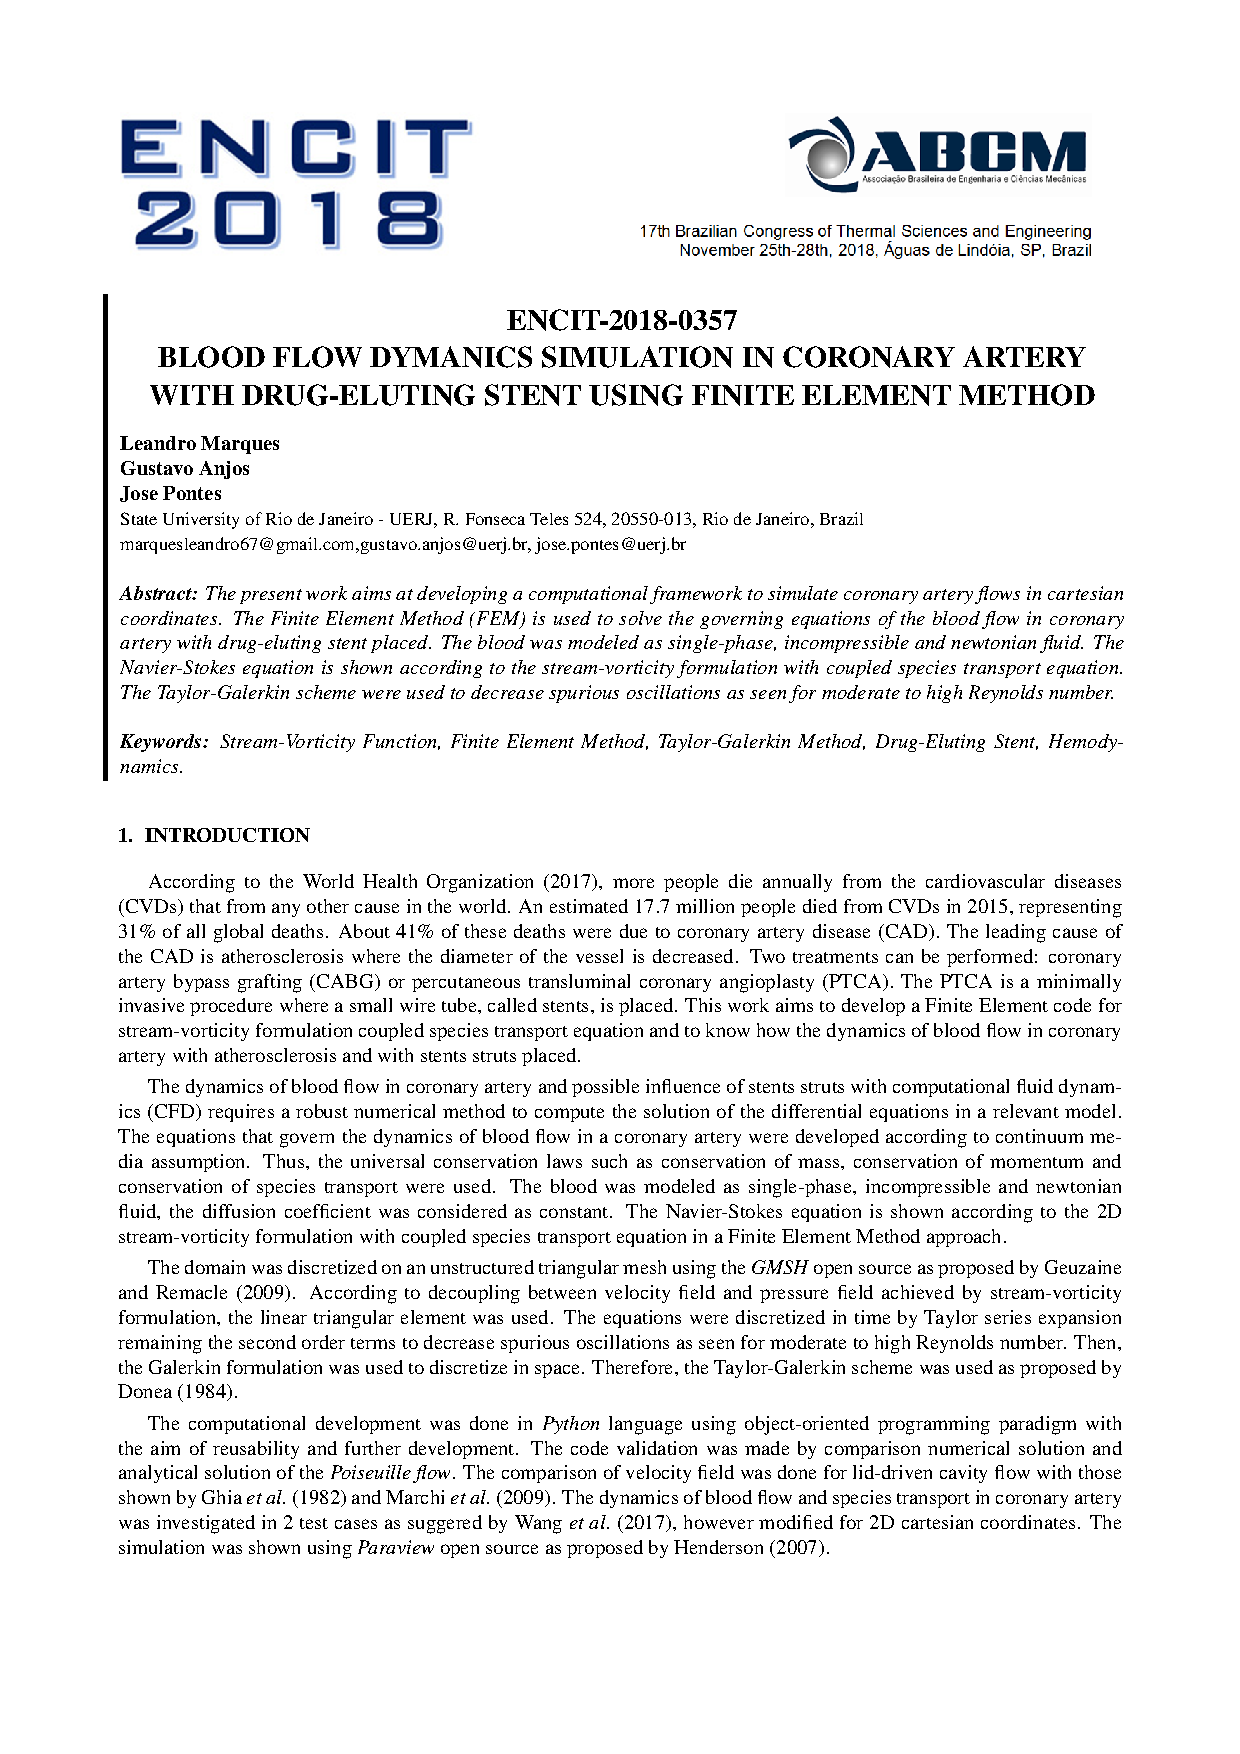
\includepdf[scale=0.95,pages=-]{./04_app/ENCIT2018_final.pdf}
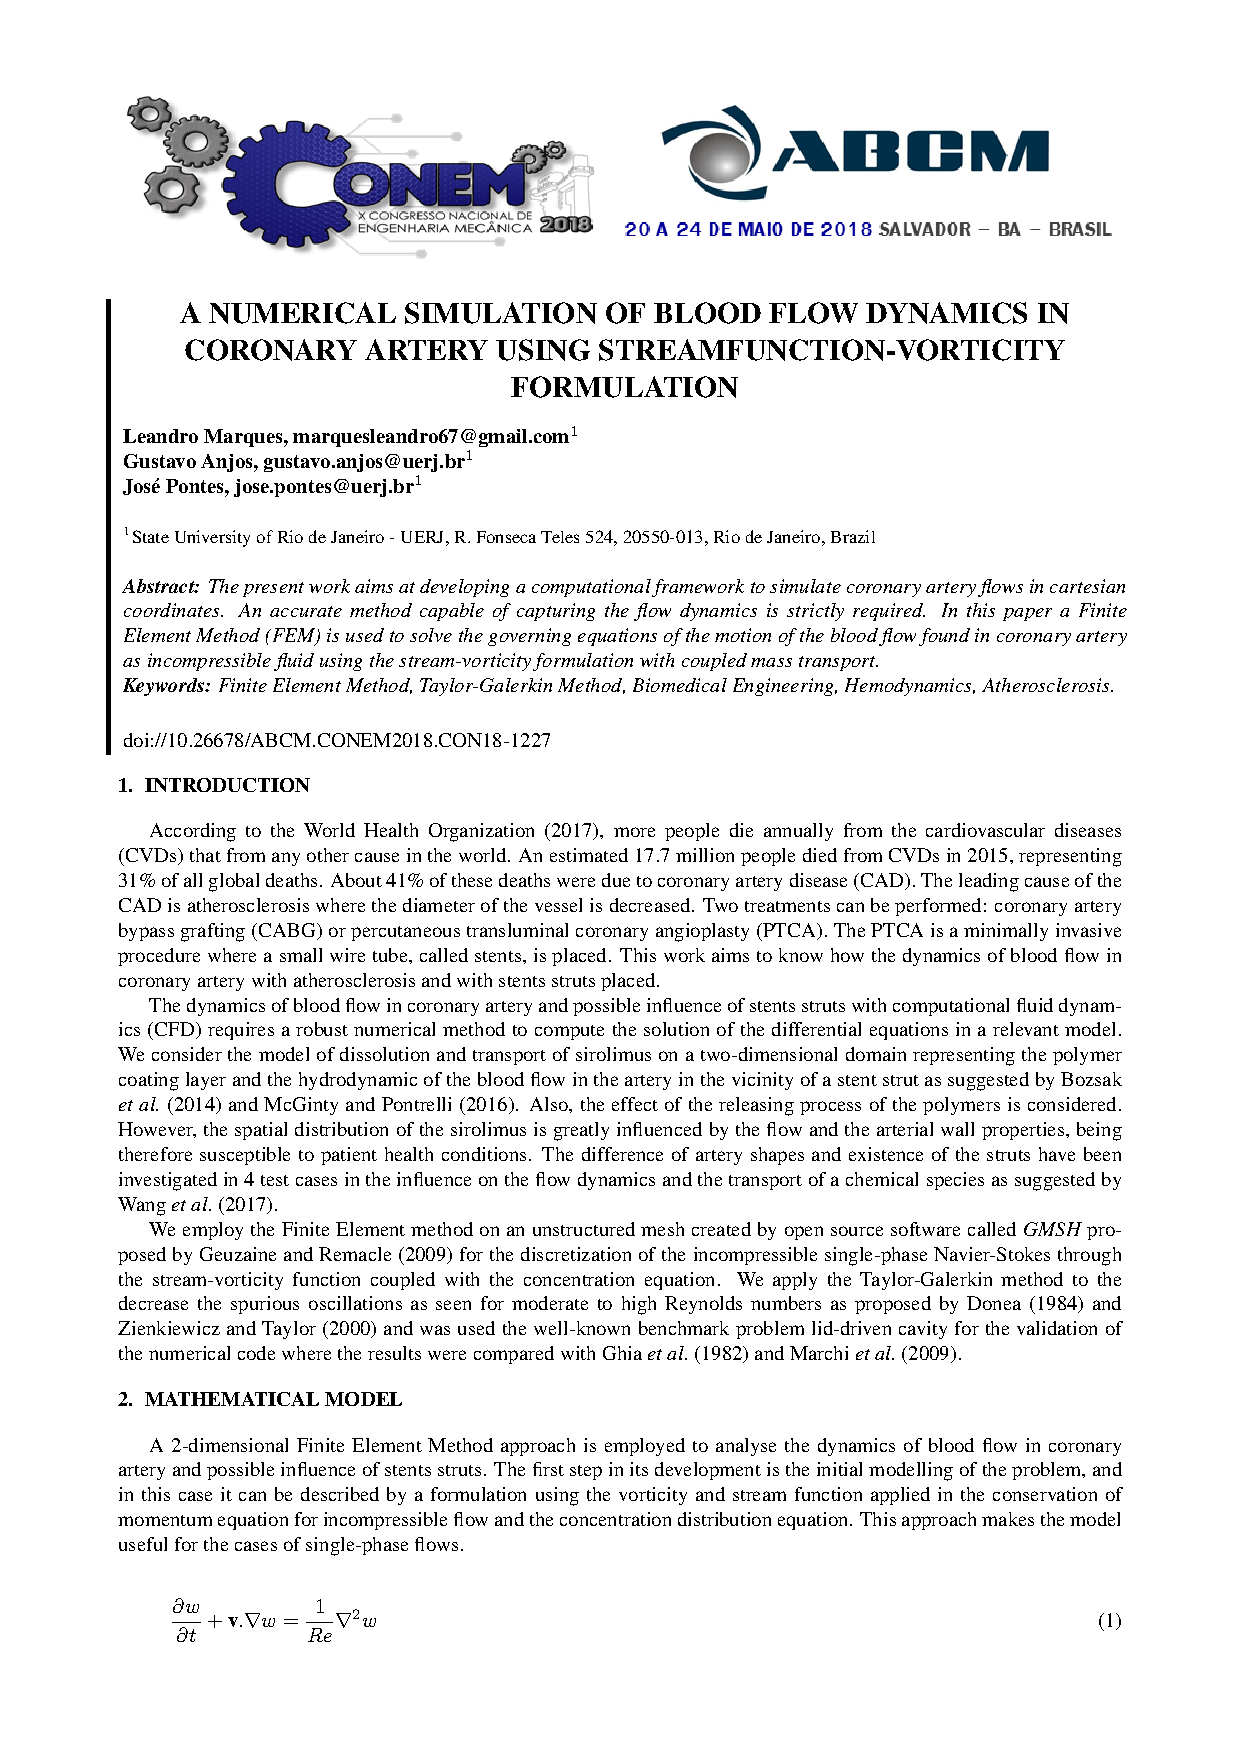
\includepdf[scale=0.95,pages=-]{./04_app/CONEM2018.pdf}
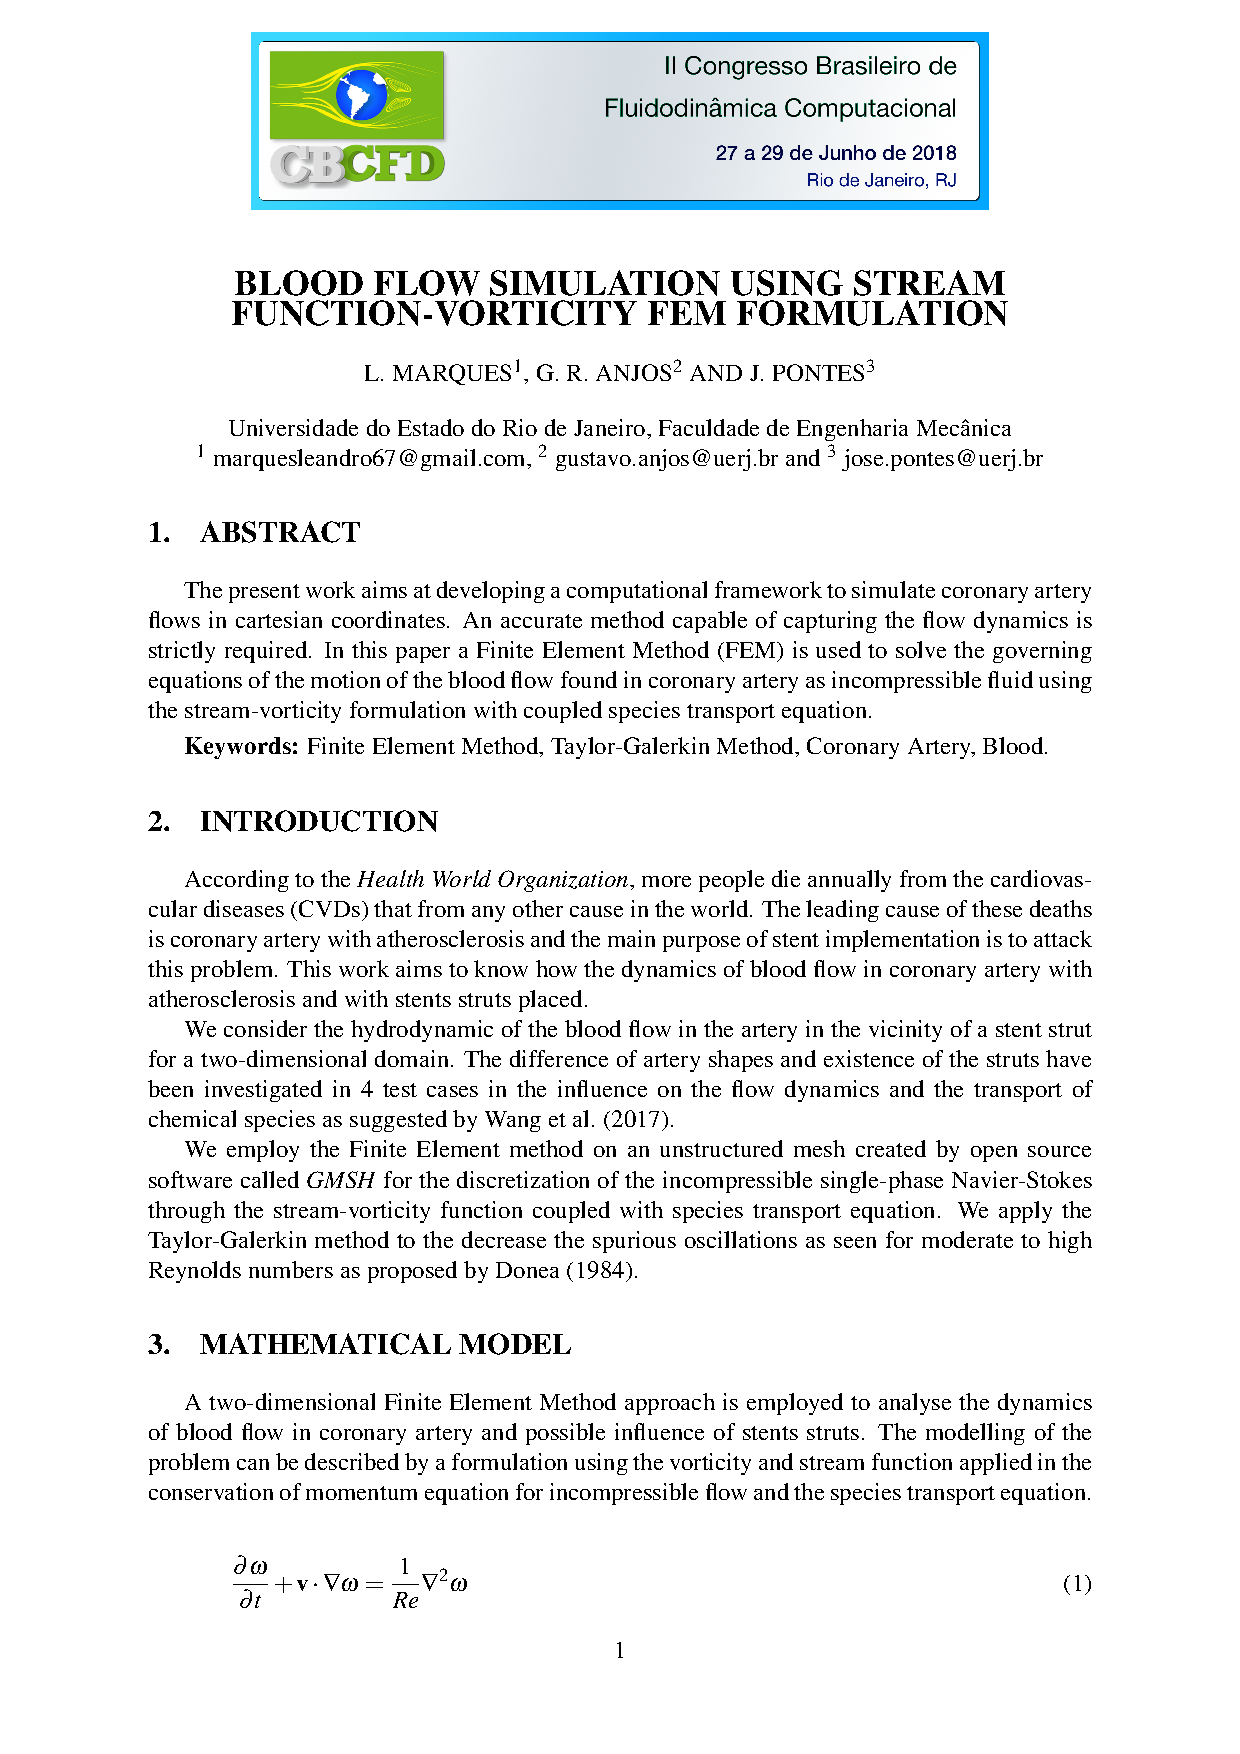
\includepdf[scale=0.95,pages=-]{./04_app/CBCFD.pdf}

\null\newpage
